\section{Virtual Machines Preparation}

\centeredlargetext{white}{black}{
Virtual Machines Preparation
}

\begin{frame}
\frametitle{Virtual Machines Preparation}
\begin{itemize}
\item Get DVD / USB Memory Stick
\item Install VirtualBox from it
\item Import the VirtualMachine file
\item Boot the Virtual Machine
\item Log in
\item Get familiar with directories
\end{itemize}
\end{frame}


\begin{frame}
\frametitle{Media Content}
\framesubtitle{Directories and Files}
\begin{itemize}
\item VirtualBoxInstallers
\begin{itemize}
\item VirtualBox-4.1.2-73507-OSX.dmg (Mac)
\item VirtualBox-4.1.2-73507-Win.exe (Windows)
\item (Ubuntu Linux)
\begin{itemize}
\item virtualbox-4.1\_4.1.2-73507~Ubuntu~lucid\_amd64.deb
\item virtualbox-4.1\_4.1.2-73507~Ubuntu~lucid\_i386.deb
\item virtualbox-4.1\_4.1.2-73507~Ubuntu~maverick\_amd64.deb
\item virtualbox-4.1\_4.1.2-73507~Ubuntu~maverick\_i386.deb
\item virtualbox-4.1\_4.1.2-73507~Ubuntu~natty\_amd64.deb
\item virtualbox-4.1\_4.1.2-73507~Ubuntu~natty\_i386.deb
\item \ldots
\end{itemize}
\end{itemize}
\pause
\item VirtualMachine
\begin{itemize}
\item  ITKv4-disk1.vmdk
\item  ITKv4.ovf
\end{itemize}
\end{itemize}
\end{frame}

\begin{frame}
\frametitle{Install VirtualBox}
\begin{itemize}
\item Select the installer for your platform
\item Run it
\end{itemize}
\end{frame}

\begin{frame}
\frametitle{Alternative Linux Installation}
\begin{itemize}
\item  You can also install VirtualBox by doing:
\item  sudo apt-get install virtualbox-ose-qt
\end{itemize}
\end{frame}

\begin{frame}
\frametitle{Importing the Virtual Machine}
\begin{itemize}
\item Run VirtualBox
\item In ``File'' Menu select ``Import Appliance''
\item Provide the filename in the DVD / USB stick ``VirtualMachine/ITKv4.ovf"
\item A progress bar will appear, and when it finishes you should see:
\end{itemize}
\begin{center}
  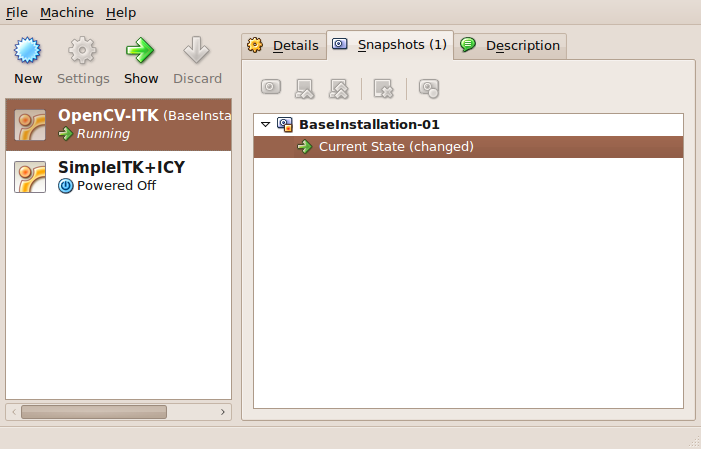
\includegraphics[width=0.5\paperwidth]{../Art/Screenshot-VirtualBox-OSE-01.png}
\end{center}
\end{frame}


\centeredlargetext{white}{black}{
We will get back...
}

